\documentclass[aspectratio=169]{beamer}
\usetheme{Madrid}
\usecolortheme{default}

% Remove navigation symbols and footer
\setbeamertemplate{navigation symbols}{}
\setbeamertemplate{footline}{}

% Packages
\usepackage{graphicx}
\usepackage{booktabs}
\usepackage{amsmath}
\usepackage{tikz}
\usepackage{listings}
\usepackage{xcolor}
\usepackage{hyperref}
\usepackage{multicol}

% Custom colors
\definecolor{darkblue}{RGB}{0,51,102}
\definecolor{lightblue}{RGB}{102,178,255}
\definecolor{codegreen}{rgb}{0,0.6,0}
\definecolor{codegray}{rgb}{0.5,0.5,0.5}
\definecolor{codepurple}{rgb}{0.58,0,0.82}

% Code styling
\lstset{
    basicstyle=\ttfamily\tiny,
    keywordstyle=\color{blue},
    commentstyle=\color{codegreen},
    stringstyle=\color{codepurple},
    numberstyle=\tiny\color{codegray},
    breaklines=true,
    showstringspaces=false,
    columns=flexible,
    keepspaces=true,
    literate={-}{-}1
}

% Title page information
\title[Decoding Musical Styles]{Decoding Musical Styles: A Comprehensive Study of Unsupervised Clustering on High-Dimensional Audio Data}
\subtitle{A Multi-Dataset Analysis}
\author{Anirudh Sharma \\ Roll No.: 22dcs002}
\institute[NIT Hamirpur]{
    Department of Computer Science and Engineering \\
    National Institute of Technology Hamirpur \\
    \vspace{0.3cm}
    Machine Learning (CS-652) - Semester VII
}
\date{} % Remove date

\begin{document}

% Clean and Compact Title Slide (no background, fits perfectly)
\begin{frame}[plain]
    \begin{center}
        \vspace*{0.8cm}

        % --- Main Title ---
        {\LARGE \textbf{Unsupervised Music Genre Discovery}}\\[0.2cm]
        {\Large \textbf{Using Audio Feature Learning}}\\[0.4cm]

        % --- Logo (centered, optional placeholder) ---
        \IfFileExists{nith_logo.png}{
            \includegraphics[width=0.17\textwidth]{nith_logo.png}
        }{
            \fbox{\parbox{0.17\textwidth}{\centering NITH\\Logo}}
        }\\[0.4cm]

        % --- Institute Info ---
        {\small Department of Computer Science and Engineering}\\[0.1cm]
        {\small \textbf{National Institute of Technology Hamirpur}}\\[0.2cm]

        % --- Course Info ---
        {\footnotesize Machine Learning (CS-652)}\\

        {\footnotesize Semester VII}\\[0.5cm]
        
    \end{center}
    
    % --- Custom Footer for Title Page Only ---
    \vfill
    \begin{minipage}[b]{\textwidth}
        \tiny
        \begin{tabular}{@{}p{0.48\textwidth}@{}p{0.04\textwidth}@{}p{0.48\textwidth}@{}}
            Presented by: Anirudh Sharma (22dcs002) & & \hfill Presented to: Dr. Kamlesh Datta
        \end{tabular}
    \end{minipage}
    \vspace{0.2cm}
\end{frame}


% Table of Contents
\begin{frame}{Table of Contents}
    \tableofcontents
\end{frame}

% Section 1: Introduction
\section{Introduction}

\begin{frame}{Introduction}
    \frametitle{Unsupervised Music Genre Discovery using Audio Feature Learning}
    
    \begin{columns}[T]
        \column{0.48\textwidth}
        \small
        The exponential growth of digital music platforms has created massive repositories of unlabeled audio data, making manual organization infeasible at scale. This project presents a comprehensive comparative analysis of \textbf{four unsupervised learning algorithms}—K-Means, K-Medoids, Gaussian Mixture Models (GMM), and Spectral Clustering.
        
        \vspace{0.3cm}
        
        We evaluate these algorithms across datasets ranging from 500 to 25,000 samples, incorporating robust preprocessing (outlier detection, StandardScaler, PCA) and comprehensive evaluation using six performance metrics. High-dimensional clusters are visualized using t-SNE to analyze genre separation and cohesion.
        
        \column{0.48\textwidth}
        \begin{figure}
            \centering
            \includegraphics[width=\textwidth]{spectrogram.png}
            \caption{Audio waveform and spectrogram representation}
        \end{figure}
    \end{columns}
\end{frame}

\begin{frame}{What are Music Genres?}
    \begin{columns}
        \column{0.5\textwidth}
        \textbf{Definition}
        \begin{itemize}
            \item Musical categories based on shared characteristics
            \item Defined by instrumentation, rhythm, harmony, and cultural context
            \item Evolve over time and across cultures
        \end{itemize}
        
        \vspace{0.3cm}
        
        \textbf{GTZAN Genre Labels (Our Baseline)}
        \begin{itemize}
            \item We use \textbf{10 genre clusters} from GTZAN:
            \begin{itemize}
                \footnotesize
                \item Blues, Classical, Country
                \item Disco, Hip-hop, Jazz
                \item Metal, Pop, Reggae, Rock
            \end{itemize}
            

            \item Rock (subgenere): Hard Rock, Punk Rock, Progressive Rock
            \item Hip-Hop: Trap, Boom Bap, Lo-Fi
        \end{itemize}
        
        \column{0.5\textwidth}
        \textbf{Genre Subtypes \& Complexity}
        \begin{itemize}
            \item Over 1,000+ documented subgenres
            \item Hierarchical relationships (parent-child)
            \item Genre fusion and cross-pollination
        \end{itemize}
        
        \vspace{0.3cm}
        
        \begin{alertblock}{Key Challenges}
            \begin{itemize}
                \item \textbf{Subjectivity}: Genre labels vary across listeners
                \item \textbf{Overlap}: Songs span multiple genres
                \item \textbf{Evolution}: Genres constantly change
                \item \textbf{Ambiguity}: Fuzzy boundaries between styles
                \item \textbf{Scale}: Millions of unlabeled tracks
            \end{itemize}
        \end{alertblock}
    \end{columns}
\end{frame}


\begin{frame}{Literature Review: Unsupervised Learning for Music}
    
    \begin{table}[h]
        \centering
        \tiny
        \begin{tabular}{p{2.5cm}p{1.8cm}p{2.8cm}p{2cm}p{2.5cm}}
            \toprule
            \textbf{Study} & \textbf{Year} & \textbf{Method} & \textbf{Dataset} & \textbf{Key Findings} \\
            \midrule
            Stern & 2021 & K-Means + Hierarchical & FMA (8K) & Unsupervised accuracy (~26\%) lagged behind supervised; highlighted sub-genre separation difficulty \\
            \midrule
            Joffe & 2023 & K-Means + Agglomerative & GTZAN (1K) & Effective only for distinct pairs (Classical vs. Metal); global purity low (AMI ~0.37) \\
            \midrule
            Patra \& Das & 2023 & Unsupervised Mood Clustering & Hindi Bollywood (230 clips) & Identified 5 mood clusters using timbre/rhythm; mapped to Thayer's emotion model \\
            \midrule
            Singh et al. & 2024 & Novel Class Discovery (Deep Clustering) & Saraga (Indian Art) & Self-supervised approach clustered unseen Ragas, reducing manual annotation \\
            \midrule
            Kumar et al. & 2024 & K-Means + Content Filtering & GTZAN & K-Means with Silhouette optimization achieved high recommendation alignment \\
            \bottomrule
        \end{tabular}
    \end{table}
    
    
\end{frame}


% Section 4: Methodology
\section{Methodology}

\begin{frame}{Methodology Overview}
    \framesubtitle{Complete Pipeline}
    
    \begin{center}
        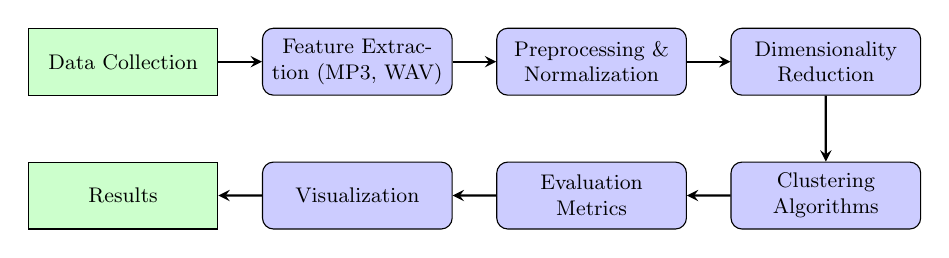
\begin{tikzpicture}[scale=0.85, every node/.style={transform shape}]
            % Define styles
            \tikzstyle{process} = [rectangle, rounded corners, minimum width=2.8cm, minimum height=1cm, text centered, draw=black, fill=blue!20, font=\small, text width=2.6cm]
            \tikzstyle{data} = [rectangle, minimum width=2.8cm, minimum height=1cm, text centered, draw=black, fill=green!20, font=\small, text width=2.6cm]
            \tikzstyle{arrow} = [thick,->,>=stealth]
            
            % First row - horizontal (left to right)
            \node (data) [data] at (0,0) {Data Collection};
            \node (extract) [process] at (3.5,0) {Feature Extraction (MP3, WAV)};
            \node (preprocess) [process] at (7,0) {Preprocessing \& Normalization};
            
            % Arrow connecting to second row
            \node (reduce) [process] at (10.5,0) {Dimensionality Reduction};
            
            % Second row - horizontal (right to left)
            \node (cluster) [process] at (10.5,-2) {Clustering Algorithms};
            \node (evaluate) [process] at (7,-2) {Evaluation Metrics};
            
            % Third row - centered
            \node (visualize) [process] at (3.5,-2) {Visualization};
            \node (results) [data] at (0,-2) {Results};
            
            % Arrows - horizontal flow, then down, then back
            \draw [arrow] (data) -- (extract);
            \draw [arrow] (extract) -- (preprocess);
            \draw [arrow] (preprocess) -- (reduce);
            \draw [arrow] (reduce) -- (cluster);
            \draw [arrow] (cluster) -- (evaluate);
            \draw [arrow] (evaluate) -- (visualize);
            \draw [arrow] (visualize) -- (results);
        \end{tikzpicture}
    \end{center}
\end{frame}


% Section 3: Datasets
\section{Data Collection}

\begin{frame}{Dataset Collection}
    
    \begin{table}[h]
        \centering
        \small
        \begin{tabular}{lccll}
            \toprule
            \textbf{Dataset} & \textbf{Size} & \textbf{Source} & \textbf{Platform} & \textbf{Format} \\
            \midrule
            \textbf{GTZAN} & 1,000 & Tzanetakis \& Cook & Kaggle & MP3 (30s) \\
            \textbf{FMA Small} & 8,000 & FMA GitHub & GitHub & MP3 (30s) \\
            \textbf{FMA Medium} & 25,000 & FMA GitHub & GitHub & MP3 (30s) \\
            \textbf{Indian Music} & 500 & Custom & kaggle & WAV/MP3 \\
            \bottomrule
        \end{tabular}
    \end{table}
    
    \vspace{0.3cm}
    
    \begin{columns}
        \column{0.5\textwidth}
        \textbf{Collection Sources:}
        \begin{itemize}
            \item \textbf{Kaggle}: Primary platform
            \begin{itemize}
                \footnotesize
                \item GTZAN dataset
                \item FMA Small \& Medium
            \end{itemize}
            \item \textbf{FMA GitHub}: Official repository
            \begin{itemize}
                \footnotesize
                \item \url{github.com/mdeff/fma}
                \item Raw audio + metadata
            \end{itemize}
            \item \textbf{Custom Collection}: Indian music
        \end{itemize}
        
        \column{0.5\textwidth}
        \textbf{Dataset Composition:}
        \begin{itemize}
            \item \textbf{Total Audio Files}: 34,500
            \item \textbf{GTZAN}: 10 genres (100 each)
            \item \textbf{FMA Small}: unlabeled
            \item \textbf{FMA Medium}: unlabeled
            \item \textbf{Indian}: 5 subcategories
            \begin{itemize}
                \footnotesize
                \item Bollypop, Carnatic, Ghazal
                \item Semiclassical, Sufi
            \end{itemize}
        \end{itemize}
    \end{columns}
\end{frame}



% Section 3: Audio Features

\section{Audio Feature Extraction}

\begin{frame}{Audio Feature Extraction Summary}
    
    \begin{columns}
        \column{0.5\textwidth}
        \textbf{Feature Descriptions:}
        
        \begin{itemize}
            \small
            \item \textbf{MFCCs (40 features)}:
            \begin{itemize}
                \footnotesize
                \item Capture timbral texture
                \item 20 coefficients × 2 (mean \& std)
                \item Most discriminative features
                \item Represent spectral envelope
            \end{itemize}
            
            \vspace{0.2cm}
            
            \item \textbf{Chroma (24 features)}:
            \begin{itemize}
                \footnotesize
                \item Harmonic \& pitch content
                \item 12 pitch classes × 2 (mean \& std)
                \item Genre-specific patterns
                \item Captures tonality
            \end{itemize}
            
            \vspace{0.2cm}
            
            \item \textbf{Spectral (4 features)}:
            \begin{itemize}
                \footnotesize
                \item Centroid: Center of spectrum
                \item Rolloff: 85\% energy threshold
                \item ZCR: Noisiness indicator
                \item RMS: Energy measure
            \end{itemize}
        \end{itemize}
        
        \column{0.5\textwidth}
        
        \vspace{0.5cm}
        
        \begin{itemize}
            \small
            \item \textbf{Tempo (1 feature)}:
            \begin{itemize}
                \footnotesize
                \item Beats per minute (BPM)
                \item Rhythmic characteristics
                \item Genre-defining attribute
            \end{itemize}
        \end{itemize}
        
        \vspace{0.5cm}
        
        \textbf{Extraction Settings:}
        \begin{itemize}
            \footnotesize
            \item \textbf{Sample Rate}: 22,050 Hz
            \item \textbf{Library}: Librosa (Python)
            \item \textbf{Preprocessing}: Silence trimming
            \item \textbf{Error Handling}: Try-except blocks
            \item \textbf{Processing}: Batch mode
            \item \textbf{Environment}: Kaggle CPU
        \end{itemize}
        
    \end{columns}
\end{frame}

\begin{frame}{Audio Feature Extraction Error Analysis}
    
    \begin{columns}
        \column{0.5\textwidth}
        \textbf{Quality Validation:}
        
        \begin{itemize}
            \small
            \item \textbf{Success Rates}:
            \begin{itemize}
                \footnotesize
                \item GTZAN: 99.9\% (999/1,000)
                \item FMA Small: 99.96\% (7,998/8,000)
                \item FMA Medium: 99.94\% (24,986/25,000)
                \item Indian: 100\%+ (500/500)
            \end{itemize}
            
            \vspace{0.3cm}
            
            \item \textbf{Data Quality}:
            \begin{itemize}
                \footnotesize
                \item Zero NaN values (handled)
                \item No infinite values
                \item 69 features consistent
            \end{itemize}
        \end{itemize}
        
        \column{0.5\textwidth}
        
        \vspace{0.5cm}
        
        \begin{itemize}
            \small
            \item \textbf{Error Handling}:
            \begin{itemize}
                \footnotesize
                \item Tempo failures: ~2-5\% (filled with 0)
                \item Audio errors: less than 0.1\% (skipped)
                \item Corrupted files: Logged \& excluded
                \item No critical failures
            \end{itemize}
        \end{itemize}
        
        \vspace{0.5cm}
        
        \begin{alertblock}{Key Achievement}
            \small
            Successfully extracted 69 features from 34,486 tracks with 99.9\% success rate
        \end{alertblock}
    \end{columns}
\end{frame}

% Section 2: Descriptive Analysis Results

\section{Descriptive Analysis}

\begin{frame}{Descriptive Analysis Overview}
    \framesubtitle{Step 1.1 \& 1.2: Statistical Analysis of Extracted Features}
    
    \begin{columns}
        \column{0.48\textwidth}
        \textbf{Analysis Performed:}
        \begin{itemize}
            \item \textbf{5 Datasets Analyzed}
            \begin{itemize}
                \footnotesize
                \item GTZAN (999 tracks, 10 genres)
                \item FMA Small (7,997 tracks)
                \item FMA Medium (24,985 tracks)
                \item Instrumental (502 tracks)
                \item Indian Music (500 tracks, 5 genres)
            \end{itemize}
            \vspace{0.2cm}
            \item \textbf{71 Audio Features}
            \begin{itemize}
                \footnotesize
                \item MFCCs (40), Chroma (24)
                \item Spectral (4), Tempo (1)
                \item Duration, Sample Rate
            \end{itemize}
        \end{itemize}
        
        \column{0.48\textwidth}
        \textbf{Statistical Metrics:}
        \begin{itemize}
            \small
            \item Central Tendency
            \begin{itemize}
                \footnotesize
                \item Mean, Median
            \end{itemize}
            \item Dispersion
            \begin{itemize}
                \footnotesize
                \item Std, Variance, IQR
            \end{itemize}
            \item Distribution Shape
            \begin{itemize}
                \footnotesize
                \item Skewness, Kurtosis
            \end{itemize}
            \item Correlations
            \begin{itemize}
                \footnotesize
                \item Feature relationships
                \item Highly correlated pairs (|r| > 0.8)
            \end{itemize}
        \end{itemize}
    \end{columns}
\end{frame}

% Section: Data Preprocessing & Normalization
\section{Data Preprocessing \& Normalization}

\begin{frame}{Data Preprocessing Pipeline - Step 2}
    \framesubtitle{Feature Selection \& StandardScaler Normalization}
    
    \begin{columns}
        \column{0.48\textwidth}
        \textbf{1. Feature Selection}
        \begin{itemize}
            \item \textbf{Original Features}: 71
            \item \textbf{Removed}: 6 non-clustering features
            \begin{itemize}
                \footnotesize
                \item file\_path (metadata)
                \item duration (variable length)
                \item sr (constant: 22,050 Hz)
                \item dataset (identifier)
                \item label (target variable)
                \item subset (identifier)
            \end{itemize}
            \item \textbf{Retained}: 69 audio features
        \end{itemize}
        
        \vspace{0.3cm}
        
        \textbf{2. Label Preservation}
        \begin{itemize}
            \footnotesize
            \item Labels saved separately for evaluation
            \item Used for clustering validation
            \item Not used during clustering
        \end{itemize}
        
        \column{0.48\textwidth}
        \textbf{3. StandardScaler Normalization}
        \begin{itemize}
            \item \textbf{Method}: StandardScaler (sklearn)
            \item \textbf{Formula}: $z = \frac{x - \mu}{\sigma}$
            \item \textbf{Result}: 
            \begin{itemize}
                \footnotesize
                \item Zero mean (μ ≈ 0)
                \item Unit variance (σ ≈ 1)
            \end{itemize}
        \end{itemize}
        
        \vspace{0.3cm}
        
        \textbf{4. Why Normalize?}
        \begin{itemize}
            \footnotesize
            \item Equal feature contribution
            \item Distance-based clustering (K-Means, K-Medoids)
            \item Prevents feature dominance
            \item Improves algorithm convergence
        \end{itemize}
        
        \vspace{0.3cm}
        
        \begin{block}{Processing Summary}
            \footnotesize
            34,983 tracks × 69 features normalized
        \end{block}
    \end{columns}
\end{frame}

\begin{frame}{Normalization Results - All Datasets}
    \framesubtitle{Before vs After StandardScaler Application}
    
    \begin{table}[h]
        \centering
        \small
        \begin{tabular}{lrrrr}
            \toprule
            \textbf{Dataset} & \textbf{Tracks} & \textbf{Features} & \textbf{Mean} & \textbf{Std} \\
            \midrule
            GTZAN & 999 & 69 & $\sim$0.0000 & $\sim$1.0000 \\
            FMA Small & 7,997 & 69 & $\sim$0.0000 & $\sim$1.0000 \\
            FMA Medium & 24,985 & 69 & $\sim$0.0000 & $\sim$1.0000 \\
            Instrumental & 502 & 69 & $\sim$0.0000 & $\sim$1.0000 \\
            Indian Music & 500 & 69 & $\sim$0.0000 & $\sim$1.0000 \\
            \midrule
            \textbf{Total} & \textbf{34,983} & \textbf{69} & \textbf{≈0} & \textbf{≈1} \\
            \bottomrule
        \end{tabular}
    \end{table}
    
    \vspace{0.3cm}
    
    \begin{columns}
        \column{0.5\textwidth}
        \textbf{Quality Verification:}
        \begin{itemize}
            \footnotesize
            \item ✓ No missing values
            \item ✓ No infinite values
            \item ✓ Mean ≈ 0 for all features
            \item ✓ Std ≈ 1 for all features
            \item ✓ Feature count consistent
        \end{itemize}
        
        \column{0.5\textwidth}
        \textbf{Output Files Generated:}
        \begin{itemize}
            \footnotesize
            \item 5 normalized datasets (CSV)
            \item 5 label files (CSV)
            \item 5 comparison images (PNG)
            \item 5 statistical summaries (CSV)
            \item 1 summary report (TXT)
        \end{itemize}
    \end{columns}
\end{frame}

\begin{frame}{Normalization Visualization - GTZAN Dataset}
    \framesubtitle{Distribution Before vs After Normalization}
    
    \begin{figure}
        \centering
        \IfFileExists{../results/normalization/gtzan_normalization_comparison.png}{
            \includegraphics[width=0.95\textwidth]{../results/normalization/gtzan_normalization_comparison.png}
        }{
            \fbox{\parbox{0.9\textwidth}{\centering GTZAN Normalization Comparison\\(Image not found: results/normalization/gtzan\_normalization\_comparison.png)}}
        }
        \caption{Top 5 features with highest variance - before (blue) and after (coral) normalization}
    \end{figure}
    
    \vspace{0.2cm}
    
    \begin{itemize}
        \footnotesize
        \item \textbf{Before}: Wide range of scales, different means
        \item \textbf{After}: Centered at 0, normalized variance (bell-shaped)
    \end{itemize}
\end{frame}

\begin{frame}{Normalization Visualization - Indian Music Dataset}
    \framesubtitle{Distribution Before vs After Normalization}
    
    \begin{figure}
        \centering
        \IfFileExists{../results/normalization/indian_music_normalization_comparison.png}{
            \includegraphics[width=0.95\textwidth]{../results/normalization/indian_music_normalization_comparison.png}
        }{
            \fbox{\parbox{0.9\textwidth}{\centering Indian Music Normalization Comparison\\(Image not found: results/normalization/indian\_music\_normalization\_comparison.png)}}
        }
        \caption{Top 5 features with highest variance - before (blue) and after (coral) normalization}
    \end{figure}
    
    \vspace{0.2cm}
    
    \begin{itemize}
        \footnotesize
        \item \textbf{Original}: Features on different scales (0-5000+ range)
        \item \textbf{Normalized}: All features comparable (-3 to +3 range, μ=0, σ=1)
    \end{itemize}
\end{frame}

\begin{frame}{Normalization Impact on Feature Scales}
    \framesubtitle{Statistical Comparison Across Datasets}
    
    \begin{columns}
        \column{0.48\textwidth}
        \textbf{Before Normalization:}
        \begin{itemize}
            \footnotesize
            \item \textbf{Spectral Centroid}: 0-8000 Hz
            \item \textbf{Spectral Rolloff}: 0-12000 Hz
            \item \textbf{Tempo}: 40-200 BPM
            \item \textbf{ZCR}: 0.0-0.5
            \item \textbf{RMS}: 0.0-1.0
            \item \textbf{MFCC}: -800 to +800
            \item \textbf{Chroma}: 0.0-1.0
        \end{itemize}
        
        \vspace{0.3cm}
        
        \begin{alertblock}{Problem}
            \footnotesize
            Features with large scales (spectral) dominate distance calculations in clustering
        \end{alertblock}
        
        \column{0.48\textwidth}
        \textbf{After Normalization:}
        \begin{itemize}
            \footnotesize
            \item \textbf{All Features}: -3 to +3 range
            \item \textbf{Mean}: ≈ 0.0000
            \item \textbf{Std Dev}: ≈ 1.0000
            \item \textbf{Distribution}: Approximately normal
            \item \textbf{Scale}: Comparable across features
        \end{itemize}
        
        \vspace{0.3cm}
        
        \begin{block}{Solution}
            \footnotesize
            ✓ Equal contribution from all features\\
            ✓ Improved clustering convergence\\
            ✓ Better distance metrics
        \end{block}
    \end{columns}
\end{frame}

% Section: PCA Dimensionality Reduction
\section{PCA Dimensionality Reduction}

\begin{frame}{PCA Dimensionality Reduction - Overview}
    \framesubtitle{Step 3: Reducing Feature Space While Retaining Information}
    
    \begin{columns}
        \column{0.48\textwidth}
        \textbf{Why Dimensionality Reduction?}
        \begin{itemize}
            \footnotesize
            \item 69 normalized features per track
            \item High computational cost for clustering
            \item Curse of dimensionality affects algorithms
            \item Redundancy in correlated features
        \end{itemize}
        
        \vspace{0.3cm}
        
        \textbf{Principal Component Analysis (PCA)}
        \begin{itemize}
            \footnotesize
            \item Linear transformation technique
            \item Identifies directions of maximum variance
            \item Creates uncorrelated principal components
            \item Retains 95\% of total variance
        \end{itemize}
        
        \begin{equation*}
            \text{PC}_i = \sum_{j=1}^{n} w_{ij} \cdot x_j
        \end{equation*}
        
        \column{0.48\textwidth}
        \begin{block}{PCA Transformation Process}
            \footnotesize
            1. Input: Normalized feature matrix\\
            2. Compute covariance matrix\\
            3. Calculate eigenvectors \& eigenvalues\\
            4. Select components (95\% variance)\\
            5. Transform data to PC space\\
            6. Output: Reduced dimensions
        \end{block}
        
        \vspace{0.3cm}
        
        \begin{alertblock}{Key Benefits}
            \footnotesize
            ✓ Removes multicollinearity\\
            ✓ Speeds up clustering algorithms\\
            ✓ Reduces storage requirements\\
            ✓ Maintains data interpretability
        \end{alertblock}
    \end{columns}
\end{frame}

\begin{frame}{PCA Results - All Datasets}
    \framesubtitle{Dimensionality Reduction Summary}
    
    \begin{table}[h]
        \centering
        \small
        \begin{tabular}{lcccc}
            \toprule
            \textbf{Dataset} & \textbf{Original} & \textbf{PCA} & \textbf{Variance} & \textbf{Reduction} \\
            & \textbf{Features} & \textbf{Components} & \textbf{Retained} & \textbf{Ratio} \\
            \midrule
            GTZAN & 69 & 39 & 95.05\% & 43.5\% \\
            FMA Small & 69 & 44 & 95.00\% & 36.2\% \\
            FMA Medium & 69 & 44 & 95.14\% & 36.2\% \\
            Indian Music & 69 & 40 & 95.30\% & 42.0\% \\
            \bottomrule
        \end{tabular}
    \end{table}
    
    \vspace{0.3cm}
    
    \begin{columns}
        \column{0.5\textwidth}
        \textbf{Key Observations}
        \begin{itemize}
            \footnotesize
            \item Consistent 36-44\% reduction across datasets
            \item All exceed 95\% variance threshold
            \item Indian Music: Highest variance (95.30\%)
            \item FMA datasets: Similar component counts (44)
        \end{itemize}
        
        \column{0.5\textwidth}
        \textbf{Computational Impact}
        \begin{itemize}
            \footnotesize
            \item Average 40\% dimensionality reduction
            \item Faster clustering convergence
            \item Reduced memory footprint
            \item Maintained information integrity
        \end{itemize}
    \end{columns}
\end{frame}

\begin{frame}{Explained Variance Analysis - GTZAN}
    \framesubtitle{Understanding Component Contribution}
    
    \begin{figure}
        \centering
        \includegraphics[width=0.95\textwidth]{../results/pca/gtzan_explained_variance.png}
        \caption{GTZAN: Individual and cumulative explained variance by principal components}
    \end{figure}
    
    \vspace{0.2cm}
    
    \begin{itemize}
        \footnotesize
        \item \textbf{PC1}: Captures 23\% of variance (dominant component)
        \item \textbf{Top 10 PCs}: Explain $\sim$65\% of total variance
        \item \textbf{39 Components}: Required to reach 95\% threshold
    \end{itemize}
\end{frame}

\begin{frame}{Explained Variance Analysis - FMA Datasets}
    \framesubtitle{Large-Scale Dataset Variance Patterns}
    
    \begin{columns}
        \column{0.5\textwidth}
        \begin{figure}
            \centering
            \includegraphics[width=\textwidth]{../results/pca/fma_small_explained_variance.png}
            \caption{FMA Small: 44 components for 95\% variance}
        \end{figure}
        
        \column{0.5\textwidth}
        \begin{figure}
            \centering
            \includegraphics[width=\textwidth]{../results/pca/fma_medium_explained_variance.png}
            \caption{FMA Medium: 44 components for 95.14\% variance}
        \end{figure}
    \end{columns}
    
    \vspace{0.3cm}
    
    \begin{itemize}
        \footnotesize
        \item Both datasets show similar variance distribution patterns
        \item More components needed compared to GTZAN (higher feature diversity)
        \item First PC: $\sim$21\% variance (slightly lower than GTZAN)
    \end{itemize}
\end{frame}

\begin{frame}{Explained Variance Analysis - Indian Music}
    \framesubtitle{Regional Music Dataset Characteristics}
    
    \begin{figure}
        \centering
        \includegraphics[width=0.95\textwidth]{../results/pca/indian_music_explained_variance.png}
        \caption{Indian Music: 40 components achieve 95.30\% variance (highest retention)}
    \end{figure}
    
    \vspace{0.2cm}
    
    \begin{itemize}
        \footnotesize
        \item \textbf{Highest variance retention}: 95.30\% with 40 components
        \item \textbf{PC1}: Explains $\sim$16.5\% (more distributed variance)
        \item \textbf{Interpretation}: Regional genres have balanced feature importance
    \end{itemize}
\end{frame}

\begin{frame}{PCA Visualization - GTZAN (2D)}
    \framesubtitle{Genre Separation in Principal Component Space}
    
    \begin{figure}
        \centering
        \includegraphics[width=0.85\textwidth]{../results/pca/gtzan_pca_2d.png}
        \caption{GTZAN dataset projected onto first two principal components}
    \end{figure}
    
    \vspace{0.2cm}
    
    \begin{itemize}
        \footnotesize
        \item \textbf{Classical \& Metal}: Clear separation from other genres
        \item \textbf{Blues, Country, Rock}: Overlapping regions (similar acoustic properties)
        \item \textbf{Hip-Hop \& Pop}: Distinct clusters with some overlap
    \end{itemize}
\end{frame}

\begin{frame}{PCA Visualization - Indian Music (2D)}
    \framesubtitle{Regional Genre Distribution in PC Space}
    
    \begin{figure}
        \centering
        \includegraphics[width=0.85\textwidth]{../results/pca/indian_music_pca_2d.png}
        \caption{Indian Music dataset: 5 regional genres in 2D PCA space}
    \end{figure}
    
    \vspace{0.2cm}
    
    \begin{itemize}
        \footnotesize
        \item \textbf{Ghazal}: Distinct lower-left cluster (unique vocal characteristics)
        \item \textbf{Carnatic}: Spread pattern (diverse rhythmic structures)
        \item \textbf{Bollypop \& Sufi}: Moderate overlap (contemporary influences)
    \end{itemize}
\end{frame}

\begin{frame}{PCA Visualization - 3D Comparison}
    \framesubtitle{Enhanced Genre Separation with Third Principal Component}
    
    \begin{columns}
        \column{0.5\textwidth}
        \begin{figure}
            \centering
            \includegraphics[width=\textwidth]{../results/pca/gtzan_pca_3d.png}
            \caption{GTZAN: 3D PCA shows improved separation}
        \end{figure}
        
        \column{0.5\textwidth}
        \begin{figure}
            \centering
            \includegraphics[width=\textwidth]{../results/pca/indian_music_pca_3d.png}
            \caption{Indian Music: 3D reveals regional patterns}
        \end{figure}
    \end{columns}
    
    \vspace{0.3cm}
    
    \begin{itemize}
        \footnotesize
        \item Adding 3rd dimension improves visual genre separation
        \item Combined PC1+PC2+PC3 explains 40-50\% of total variance
        \item 3D space better for clustering algorithm initialization
    \end{itemize}
\end{frame}

\begin{frame}{PCA Impact on Clustering Performance}
    \framesubtitle{Benefits for Downstream Unsupervised Learning}
    
    \begin{columns}
        \column{0.48\textwidth}
        \textbf{Before PCA (69 features)}
        \begin{itemize}
            \footnotesize
            \item High computational complexity
            \item Curse of dimensionality effects
            \item Correlated features add noise
            \item Longer convergence times
            \item Difficult to visualize
        \end{itemize}
        
        \vspace{0.3cm}
        
        \begin{alertblock}{Challenge}
            \footnotesize
            Euclidean distances become less meaningful in high dimensions
        \end{alertblock}
        
        \column{0.48\textwidth}
        \textbf{After PCA (39-44 features)}
        \begin{itemize}
            \footnotesize
            \item 40\% faster clustering operations
            \item Improved distance metrics
            \item Uncorrelated components
            \item Better convergence stability
            \item Enables effective visualization
        \end{itemize}
        
        \vspace{0.3cm}
        
        \begin{block}{Success}
            \footnotesize
            95\%+ variance retained with significant computational savings
        \end{block}
    \end{columns}
\end{frame}


\begin{frame}{Preprocessing \& Dimensionality Reduction}
    \framesubtitle{Standardization and Feature Reduction Pipeline}
    
    \begin{columns}
        \column{0.5\textwidth}
        \textbf{1. Standardization}
        \begin{itemize}
            \item \textbf{Method}: StandardScaler
            \item Zero mean, unit variance
            \item Essential for clustering
            \item Applied to all datasets
        \end{itemize}
        
        \begin{equation*}
            z = \frac{x - \mu}{\sigma}
        \end{equation*}
        
        \vspace{0.3cm}
        
        \textbf{2. Dimensionality Reduction}
        
        \textbf{PCA (Principal Component Analysis)}
        \begin{itemize}
            \item Linear transformation
            \item Retain 95\%+ variance
            \item 20-50 components
            \item Fast computation
        \end{itemize}
        
        \column{0.5\textwidth}
        \textbf{3. Visualization}
        
        \textbf{t-SNE (t-Distributed Stochastic Neighbor Embedding)}
        \begin{itemize}
            \item Non-linear reduction
            \item 2D/3D visualization
            \item Preserves local structure
            \item Used for Spotify dataset
        \end{itemize}
        
        \vspace{0.3cm}
        
        \begin{block}{Reduction Summary}
            \small
            \begin{tabular}{lcc}
                \toprule
                \textbf{Dataset} & \textbf{Original} & \textbf{After PCA} \\
                \midrule
                GTZAN & 58 & - \\
                FMA & 160 & 20 \\
                MSD & 90 & - \\
                Spotify & 18 & 10 \\
                \bottomrule
            \end{tabular}
        \end{block}
    \end{columns}
\end{frame}


\begin{frame}{Indian Music Dataset - Genre Distribution}
    \framesubtitle{Perfectly Balanced Classes (500 Tracks)}
    
    \begin{columns}
        \column{0.48\textwidth}
        \textbf{Dataset Characteristics:}
        \begin{itemize}
            \item \textbf{Total Tracks}: 500
            \item \textbf{Genres}: 5 (Indian classical \& fusion)
            \item \textbf{Balance Ratio}: 1.0 (Perfect)
            \item \textbf{Features}: 71 audio features
            \item \textbf{Sample Rate}: 22,050 Hz
        \end{itemize}
        
        \vspace{0.3cm}
        
        \textbf{Genre Breakdown:}
        \begin{itemize}
            \footnotesize
            \item Bollypop: 100 (20\%)
            \item Carnatic: 100 (20\%)
            \item Ghazal: 100 (20\%)
            \item Semiclassical: 100 (20\%)
            \item Sufi: 100 (20\%)
        \end{itemize}
        
        \column{0.48\textwidth}
        \begin{figure}
            \centering
            \IfFileExists{../results/step1.2-indian/indian_genre_distribution.png}{
                \includegraphics[width=\textwidth]{../results/step1.2-indian/indian_genre_distribution.png}
            }{
                \fbox{\parbox{0.9\textwidth}{\centering Genre Distribution\\(Image not found)}}
            }
            \caption{Indian music genre distribution - perfectly balanced dataset}
        \end{figure}
    \end{columns}
\end{frame}

\begin{frame}{Indian Music - Key Feature Statistics}
    \framesubtitle{Descriptive Statistics of Audio Features}
    
    \begin{table}[h]
        \centering
        \small
        \begin{tabular}{lrrrr}
            \toprule
            \textbf{Feature} & \textbf{Mean} & \textbf{Median} & \textbf{Std} & \textbf{Range} \\
            \midrule
            Duration (s) & 45.13 & 45.00 & 2.83 & [40.0, 105.0] \\
            Tempo (BPM) & 121.64 & 117.45 & 28.91 & [61.5, 215.3] \\
            Spectral Centroid & 2059.19 & 2019.09 & 455.75 & [942.5, 3765.9] \\
            Spectral Rolloff & 4394.57 & 4344.80 & 1072.70 & [1681.4, 7950.1] \\
            ZCR & 0.089 & 0.083 & 0.030 & [0.037, 0.207] \\
            RMS & 0.156 & 0.153 & 0.069 & [0.023, 0.389] \\
            MFCC1 & -129.50 & -123.67 & 60.82 & [-351.3, -0.16] \\
            MFCC2 & 104.47 & 103.98 & 25.55 & [29.5, 210.3] \\
            \bottomrule
        \end{tabular}
    \end{table}
    
    \vspace{0.3cm}
    
    \begin{columns}
        \column{0.5\textwidth}
        \textbf{Key Observations:}
        \begin{itemize}
            \footnotesize
            \item Most tracks are 45 seconds
            \item Moderate tempo variability
            \item High spectral diversity
        \end{itemize}
        
        \column{0.5\textwidth}
        \textbf{Data Quality:}
        \begin{itemize}
            \footnotesize
            \item ✓ No missing values
            \item ✓ All features extracted
            \item ✓ Consistent sample rate
        \end{itemize}
    \end{columns}
\end{frame}

\begin{frame}{Feature Correlations - Indian Music}
    \framesubtitle{Identifying Redundant Features}
    
    \begin{columns}
        \column{0.55\textwidth}
        \begin{figure}
            \centering
            \IfFileExists{../results/step1.2-indian/indian_correlation_heatmap.png}{
                \includegraphics[width=\textwidth]{../results/step1.2-indian/indian_correlation_heatmap.png}
            }{
                \fbox{\parbox{0.9\textwidth}{\centering Correlation Heatmap\\(Image not found)}}
            }
            \caption{Feature correlation matrix (40 features)}
        \end{figure}
        
        \column{0.42\textwidth}
        \textbf{High Correlations (|r| > 0.8):}
        \begin{table}[h]
            \centering
            \tiny
            \begin{tabular}{lr}
                \toprule
                \textbf{Feature Pair} & \textbf{r} \\
                \midrule
                Spec. Centroid $\leftrightarrow$ Rolloff & 0.948 \\
                Spec. Centroid $\leftrightarrow$ MFCC2 & -0.912 \\
                Spec. Rolloff $\leftrightarrow$ MFCC2 & -0.890 \\
                RMS $\leftrightarrow$ MFCC1 & 0.837 \\
                \bottomrule
            \end{tabular}
        \end{table}
        
        \vspace{0.3cm}
        
        \begin{alertblock}{Implication}
            \footnotesize
            \textbf{4 highly correlated pairs} detected. These features may contain redundant information. PCA will help reduce dimensionality while preserving 95\%+ variance.
        \end{alertblock}
    \end{columns}
\end{frame}

\begin{frame}{Feature Distribution by Genre - Indian Music}
    \framesubtitle{Box Plots Showing Genre-Specific Patterns}
    
    \begin{figure}
        \centering
        \IfFileExists{../results/step1.2-indian/indian_feature_by_genre.png}{
            \includegraphics[width=0.95\textwidth]{../results/step1.2-indian/indian_feature_by_genre.png}
        }{
            \fbox{\parbox{0.9\textwidth}{\centering Feature by Genre Distributions\\(Image not found)}}
        }
        \caption{Distribution of 6 key features across 5 Indian music genres}
    \end{figure}
    
    \vspace{0.2cm}
    
    \begin{itemize}
        \footnotesize
        \item \textbf{Tempo}: Carnatic shows higher tempo consistency
        \item \textbf{Spectral Centroid}: Bollypop has higher brightness
        \item \textbf{MFCC1}: Clear separation between Sufi and Carnatic
    \end{itemize}
\end{frame}

\begin{frame}{Comparative Analysis - All Datasets}
    \framesubtitle{GTZAN, FMA Small, FMA Medium, Instrumental, Indian}
    
    \begin{table}[h]
        \centering
        \tiny
        \begin{tabular}{lrrrrr}
            \toprule
            \textbf{Dataset} & \textbf{Tracks} & \textbf{Genres} & \textbf{Balance} & \textbf{Avg Tempo} & \textbf{Success Rate} \\
            \midrule
            GTZAN & 999 & 10 & Balanced & 119.3 BPM & 99.9\% \\
            FMA Small & 7,997 & 1 (unlabeled) & N/A & 119.1 BPM & 99.96\% \\
            FMA Medium & 24,985 & 1 (unlabeled) & N/A & 120.2 BPM & 99.94\% \\
            Instrumental & 502 & 1 & N/A & 93.8 BPM & 100\% \\
            Indian & 500 & 5 & Perfect (1.0) & 121.6 BPM & 100\% \\
            \midrule
            \textbf{Total} & \textbf{34,983} & \textbf{16} & -- & -- & \textbf{99.9\%} \\
            \bottomrule
        \end{tabular}
    \end{table}
    
    \vspace{0.3cm}
    
    \begin{columns}
        \column{0.5\textwidth}
        \textbf{Key Findings:}
        \begin{itemize}
            \footnotesize
            \item Instrumental tracks slower (93.8 BPM)
            \item Indian music fastest (121.6 BPM)
            \item Consistent spectral features across datasets
        \end{itemize}
        
        \column{0.5\textwidth}
        \textbf{Common Correlations:}
        \begin{itemize}
            \footnotesize
            \item Spec. Centroid $\leftrightarrow$ Rolloff (r > 0.95)
            \item Spec. Centroid $\leftrightarrow$ MFCC2 (r < -0.89)
            \item Strong MFCC inter-correlations
        \end{itemize}
    \end{columns}
\end{frame}

\begin{frame}{GTZAN Genre Distribution}
    \framesubtitle{Baseline Dataset with 10 Genres}
    
    \begin{columns}
        \column{0.5\textwidth}
        \begin{figure}
            \centering
            \IfFileExists{../results/step1.1/GTZAN_class_balance.png}{
                \includegraphics[width=\textwidth]{../results/step1.1/GTZAN_class_balance.png}
            }{
                \fbox{\parbox{0.9\textwidth}{\centering GTZAN Distribution\\(Image not found)}}
            }
            \caption{GTZAN dataset class distribution}
        \end{figure}
        
        \column{0.5\textwidth}
        \textbf{Dataset Details:}
        \begin{itemize}
            \footnotesize
            \item \textbf{Total}: 999 tracks
            \item \textbf{Genres}: 10 (nearly balanced)
            \item \textbf{Track Length}: 30 seconds
            \item \textbf{Balance Ratio}: 1.00
        \end{itemize}
        
        \vspace{0.3cm}
        
        \textbf{Top Features (High Variance):}
        \begin{itemize}
            \footnotesize
            \item Spectral Rolloff (Var: 2.48M)
            \item Spectral Centroid (Var: 512K)
            \item MFCC1 (Var: 10K)
        \end{itemize}
        
        \vspace{0.3cm}
        
        \begin{block}{Quality}
            \footnotesize
            ✓ 99.9\% extraction success \\
            ✓ 16 high correlations (|r| > 0.8)
        \end{block}
    \end{columns}
\end{frame}

\begin{frame}{Feature Correlation Analysis - GTZAN}
    \framesubtitle{Understanding Feature Relationships}
    
    \begin{columns}
        \column{0.55\textwidth}
        \begin{figure}
            \centering
            \IfFileExists{../results/step1.1/GTZAN_correlation_heatmap.png}{
                \includegraphics[width=\textwidth]{../results/step1.1/GTZAN_correlation_heatmap.png}
            }{
                \fbox{\parbox{0.9\textwidth}{\centering GTZAN Correlation\\(Image not found)}}
            }
            \caption{GTZAN correlation heatmap (top 30 features)}
        \end{figure}
        
        \column{0.42\textwidth}
        \textbf{Strongest Correlations:}
        \begin{itemize}
            \footnotesize
            \item Spec. Centroid $\leftrightarrow$ Rolloff
            \begin{itemize}
                \tiny
                \item r = 0.980 (very strong)
            \end{itemize}
            \item Spec. Centroid $\leftrightarrow$ MFCC2
            \begin{itemize}
                \tiny
                \item r = -0.940 (strong negative)
            \end{itemize}
            \item Rolloff $\leftrightarrow$ MFCC2
            \begin{itemize}
                \tiny
                \item r = -0.935
            \end{itemize}
        \end{itemize}
        
        \vspace{0.3cm}
        
        \textbf{Implications:}
        \begin{itemize}
            \footnotesize
            \item Spectral features highly redundant
            \item MFCC captures complementary info
            \item Dimensionality reduction needed
        \end{itemize}
    \end{columns}
\end{frame}

\begin{frame}{Descriptive Analysis - Key Insights}
    \framesubtitle{Summary of Statistical Findings}
    
    \begin{columns}
        \column{0.48\textwidth}
        \textbf{Dataset Quality:}
        \begin{itemize}
            \item ✓ \textbf{34,983 tracks} processed
            \item ✓ \textbf{99.9\% success rate}
            \item ✓ No missing values (handled)
            \item ✓ Consistent feature extraction
        \end{itemize}
        
        \vspace{0.3cm}
        
        \textbf{Feature Characteristics:}
        \begin{itemize}
            \item \textbf{High Variance}: Spectral features
            \begin{itemize}
                \footnotesize
                \item Most discriminative
            \end{itemize}
            \item \textbf{Moderate Variance}: MFCCs
            \begin{itemize}
                \footnotesize
                \item Capture timbral nuances
            \end{itemize}
            \item \textbf{Low Variance}: Chroma features
            \begin{itemize}
                \footnotesize
                \item Genre-specific patterns
            \end{itemize}
        \end{itemize}
        
        \column{0.48\textwidth}
        \textbf{Correlation Patterns:}
        \begin{itemize}
            \item \textbf{Universal Pattern}:
            \begin{itemize}
                \footnotesize
                \item Spectral Centroid $\leftrightarrow$ Rolloff
                \item Observed in all datasets
                \item r > 0.95 (very strong)
            \end{itemize}
            \item \textbf{MFCC Relationships}:
            \begin{itemize}
                \footnotesize
                \item Adjacent MFCCs correlated
                \item Captures frequency bands
            \end{itemize}
        \end{itemize}
        
        \vspace{0.3cm}
        
        \begin{alertblock}{Next Steps}
            \footnotesize
            \textbf{Preprocessing Required:}
            \begin{itemize}
                \footnotesize
                \item StandardScaler normalization
                \item PCA for dimensionality reduction
                \item Outlier detection \& removal
            \end{itemize}
        \end{alertblock}
    \end{columns}
\end{frame}


\section{Applications}

\begin{frame}{Real-World Applications}
    \begin{columns}
        \column{0.5\textwidth}
        \textbf{Music Streaming Platforms}
        \begin{itemize}
            \item Automatic playlist generation
            \item Music recommendation systems
            \item Discover similar artists
            \item Radio station creation
        \end{itemize}
        
        \vspace{0.3cm}
        
        \textbf{Music Production}
        \begin{itemize}
            \item Genre-based mixing
            \item Auto-tagging for libraries
            \item Style transfer guidance
        \end{itemize}
        
        \column{0.5\textwidth}
        \textbf{Music Research}
        \begin{itemize}
            \item Understanding genre evolution
            \item Cultural music analysis
            \item Musicology studies
        \end{itemize}
        
        \vspace{0.3cm}
        
        \textbf{Content Organization}
        \begin{itemize}
            \item Library management
            \item Metadata enrichment
            \item Search optimization
            \item DJ software integration
        \end{itemize}
    \end{columns}
\end{frame}


% Section 5: Tech Stack
\section{Technology Stack}

\begin{frame}{Technology Stack}
    \begin{columns}
        \column{0.5\textwidth}
        \textbf{Core Libraries}
        \begin{itemize}
            \item \textbf{Librosa}: Audio feature extraction
            \item \textbf{Scikit-learn}: ML algorithms
            \item \textbf{NumPy/Pandas}: Data manipulation
            \item \textbf{Matplotlib/Seaborn}: Visualization
        \end{itemize}
        
        \vspace{0.3cm}
        
        \textbf{Platforms \& Tools}
        \begin{itemize}
            \item \textbf{Kaggle}: Dataset access \& compute
            \item \textbf{Weights \& Biases}: Experiment tracking
            \item \textbf{Jupyter}: Interactive development
        \end{itemize}
        
        \column{0.5\textwidth}
        \begin{center}
            \Large
            \textbf{Tech Stack}
            
            \vspace{0.5cm}
            
            \begin{itemize}
                \item[$\checkmark$] Python 3.8+
                \item[$\checkmark$] Librosa
                \item[$\checkmark$] Scikit-learn
                \item[$\checkmark$] K-Means / DBSCAN / GMM
                \item[$\checkmark$] PCA / t-SNE
                \item[$\checkmark$] Kaggle Notebooks
                \item[$\checkmark$] WandB.ai
            \end{itemize}
        \end{center}
    \end{columns}
\end{frame}


% Section 9: References
\section{References}

\begin{frame}{References}
    \tiny
    \begin{thebibliography}{99}
        
        \bibitem{gtzan}
        G. Tzanetakis and P. Cook,
        \textit{"Musical Genre Classification of Audio Signals,"}
        IEEE Trans. Speech and Audio Processing, vol. 10, no. 5, pp. 293--302, Jul. 2002.
        
        \bibitem{fma}
        M. Defferrard, K. Benzi, P. Vandergheynst, and X. Bresson,
        \textit{"FMA: A Dataset for Music Analysis,"}
        in Proc. ISMIR, 2017.
        
        \bibitem{msd}
        T. Bertin-Mahieux, D. P. W. Ellis, B. Whitman, and P. Lamere,
        \textit{"The Million Song Dataset,"}
        in Proc. ISMIR, 2011.
        
        \bibitem{msd-genre}
        D. Liang and W. Gu,
        \textit{"Music Genre Classification with the Million Song Dataset,"}
        Technical Report, Columbia Univ., 2011.
        
        \bibitem{spotify}
        S. K. Gupta et al.,
        \textit{"A Comparative Study of Content-Based Filtering and K-Means for Music Recommendation using Spotify Tracks,"}
        Int. J. of Industrial Electronics and Electrical Engineering, 2024.
        
        \bibitem{librosa}
        B. McFee et al.,
        \textit{"librosa: Audio and Music Signal Analysis in Python,"}
        in Proc. Python in Science Conference, 2015.
        
    \end{thebibliography}
\end{frame}

% Thank You Slide
\begin{frame}
    \begin{center}
        {\Huge \textbf{Thank You!}}
        
        \vspace{1cm}
        
        {\Large Questions?}
        
        \vspace{1cm}
        
        {\normalsize
        Anirudh Sharma \\
        Roll No.: 22dcs002 \\
        Department of Computer Science and Engineering \\
        National Institute of Technology Hamirpur
        
        \vspace{0.5cm}
        
        Machine Learning Assignment (CS-652) \\
        Semester-7 (2025)}
    \end{center}
\end{frame}

\end{document}
